

\begin{frame}
\thetitle{Advanced Topics}
\begin{enumerate}
\item Gumbel-Softmax: Extend reparameterization to discrete variables.
\item Flows: Optimize a tighter bound by making $q$ more flexible.
\item Importance Weighted AE:  Optimize a tighter bound through importance sampling.
\end{enumerate}
\end{frame}

\subsection{Gumbel-Softmax}
\begin{frame}
\thetitle{Gumbel-Softmax \citep{Jang2017,Maddison2017}}
\begin{itemize}
    \item Recall the reparameterization trick for estimating $\nabla_\lambda \ELBO(\theta, \lambda \param x)$ in the continuous case.
    \item What if $z$ is discrete?
\end{itemize}
\end{frame}

\begin{frame}
\thetitle{Gumbel-Softmax \citep{Jang2017,Maddison2017}}
Review: we can always use score function estimator 
\begin{align*}
 \nabla_\lambda &\ELBO(x, \theta, \lambda) = \E_{q}\Big[\log \frac{p(x, z \param \theta)}{q(z \given x \param \lambda)}\nabla_{\lambda}\log q(z \given x \param \lambda)\Big]     \\
 &= \E_{q}\Big[\Big(\log \frac{p(x, z \param \theta)}{q(z \given x \param \lambda)}- B\Big)\nabla_{\lambda}\log q(z \given x \param \lambda)\Big] 
\end{align*}

\begin{itemize}
    \item Control variate $B$ (not dependendent on $z$, but can depend on $x$). 
    \item Estimate this quantity with another neural net \citep{Mnih2014}
    \[ \Big( B(x \param \psi) -\log \frac{p(x, z \param \theta)}{q(z \given x \param \lambda)} \Big)^2 \]
    \item Can we leverage the reparameterization trick instead?
\end{itemize}
\end{frame}

\begin{frame}
\thetitle{Gumbel-Softmax \citep{Jang2017,Maddison2017}}
The ``Gumbel-Max" trick \citep{Papandreou2011}
\[ p(z_k = 1 \param \alpha) = \frac{\alpha_k}{\sum_{j=1}^K \alpha_j} \]
where $z = [0, 0, \dots, 1 , \dots, 0]$ is a one-hot vector.
Can sample from $p(z \param \alpha)$ by
\begin{enumerate}
    \item Drawing independent Gumbel noise $\epsilon =  \epsilon_1, \dots, \epsilon_K$
    \[ \epsilon_k = -\log (- \log u_k) \,\,\,\,\,\,\,\,\,\,\,\,\, u_k \sim \mathcal{U}(0, 1)\]
    \item Adding $\epsilon_k$ to $\log \alpha_k$, finding argmax, i.e.
    \[ i = \argmax_k [\log \alpha_k + \epsilon_k] \,\,\,\,\,\,\,\,\,\,\,\,\,\,\,
    z_i = 1 \]

\end{enumerate}
    More succinctly,
    \[ z = \argmax_{s \in \Delta^{K-1}}  \,\,(\log \alpha + \epsilon)^\top s = g(\epsilon, \alpha) \]
    
\end{frame}

\begin{frame}
\thetitle{Gumbel-Softmax \citep{Jang2017,Maddison2017}}
So we can reparameterize, since $z = g(\epsilon, \alpha)$ is a deterministic function applied to stochastic noise. \\ Let's try applying this:
\[ q(z_k = 1 \given x \param \lambda) = \frac{\alpha_k}{\sum_{j=1}^K \alpha_j} \,\,\,\,\,\,\,\, \alpha = \enc(x \param \lambda) \]
\begin{align*}
    \nabla_\lambda \E_{q(z \given x \param \lambda)}\Big[& \log \frac{p(x, z \param \theta)}{q(z \given x \param \lambda)}\Big] \\ &= 
    \nabla_\lambda \E_{\epsilon \sim \text{Gumbel}}\Big[ \log \frac{ p(x, g(\epsilon, \alpha) \param \theta)}{q(g(\epsilon, \alpha) \given x \param \lambda)}\Big] \\
    &=      \E_{\epsilon \sim \text{Gumbel}}\Big[\nabla_\lambda \log \frac{ p(x, g(\epsilon, \alpha) \param \theta)}{q(g(\epsilon, \alpha) \given x \param \lambda)}\Big]
\end{align*}
\end{frame}

\begin{frame}
\thetitle{Gumbel-Softmax \citep{Jang2017,Maddison2017}}
But this won't work, since
\[ z = g(\epsilon, \alpha) = \argmax_{s \in \Delta^{K-1}} (\log \alpha + \epsilon)^\top s \]
has zero gradients almost everywhere.
\\ \vspace{3mm}
Gumbel-Softmax trick: replace $\argmax$ with $\softmax$
\[ z = \softmax((\log \alpha + \epsilon)/\tau) \]
i.e.
\[ z_k = \frac{\exp((\log \alpha_k + \epsilon_k)/\tau)}{\sum_{j=1}^K \exp ((\log \alpha_j + \epsilon_j)/\tau)}\]
where $\tau$ is a temperature term. 
\end{frame}

\begin{frame}
\thetitle{Gumbel-Softmax \citep{Jang2017,Maddison2017}}
\begin{itemize}
    \item Approaches a discrete distributution as $\tau \to 0$
    \item Reparameterizable by construction
    \item Differentiable and has non-zero gradients
\end{itemize}
\center
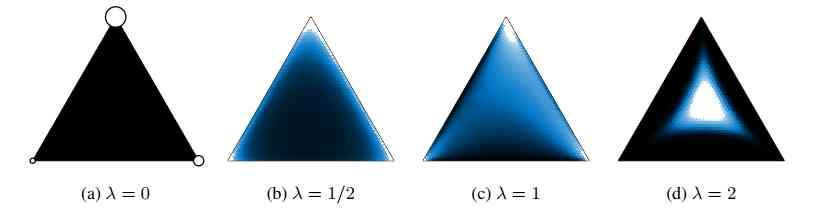
\includegraphics[scale=0.3]{pics/concrete.jpg} \\
(from \cite{Maddison2017})
\end{frame}

\begin{frame}
\thetitle{Gumbel-Softmax \citep{Jang2017,Maddison2017}}
\vspace{-5mm}
\begin{align*} 
  \nabla_\lambda& \E_{q(z \given x \param \lambda)}\Big[ \log \frac{p(x, z \param \theta)}{q(z \given x \param \lambda)}\Big] \\ &\approx 
\E_{ \epsilon \sim \text{Gumbel}}\Big[\nabla_\lambda \log \frac{ p(x, \softmax((\log \alpha + \epsilon)/\tau) \param \theta)}{q(\softmax((\log \alpha + \epsilon)/\tau) \given x \param \lambda)}\Big] 
\end{align*}
(anneal $\tau$ during training)
\begin{itemize}
\item See \cite{Maddison2017} on whether we can use the original categorical densities $p(z), q(z)$, or need to use relaxed densities $p_{\text{GS}}(z), q_{\text{GS}}(z)$.
\item Requires that $p(x \given z \param \theta)$ ``makes sense" for non-discrete $z$ (e.g. attention).
    \item Lower-variance, but biased gradient estimator. Variance $\to \infty$ as $\tau \to 0$.
\end{itemize}
\end{frame}

\subsection{Flows}

\begin{frame}
\thetitle{Flows \citep{Rezende2015,Kingma2016}}
Recall
\[ \log p(x \param \theta)  = \ELBO(\theta, \lambda; x) - \KL[q(z \given x \param \lambda)  \, \Vert \, p(z \given x \param \theta)]  \]
Bound is tight when variational posterior equals true posterior
\[ q(z \given x \param \lambda) = p(z \given x \param \theta) \implies \log p(x \param \theta) = \ELBO( \theta,  \lambda \param x) \]
We want to make $q(z \given x \param \lambda)$ as flexible as possible:
can we do better than just Gaussian?
\end{frame} 

\begin{frame}
\thetitle{Flows \citep{Rezende2015,Kingma2016}}
\textbf{Idea:} transform a sample from a simple initial variational distribution, 
\[ z_0 \sim q(z \given x \param \lambda) = \mathcal{N}(\mu, \sigma^2) \,\,\,\,\,\,\,\,\,\,\,\,\,\, \mu, \sigma^2 = \enc(x \param \lambda)\]
into a more complex one
\[ z_K = f_K \circ \dots \circ f_2 \circ f_1(z_0 \param \lambda)\]
where $f_i(z_{i-1}\param \lambda)$'s are \textbf{invertible} transformations (whose parameters are
absorbed by $\lambda$).
\end{frame} 


\begin{frame}
\thetitle{Flows \citep{Rezende2015,Kingma2016}}
Sample from final variational posterior is given by $z_K$. By the change of variables formula
\begin{align*}
\log q_K(z_K \given &x \param \lambda) = \log q(z_0 \given x \param \lambda) + 
\sum_{k=1}^K \log \Big | \frac{\partial f_k^{-1}}{\partial z_{k}}\Big |  \\
&=\underbrace{\log q(z_0 \given x \param \lambda)}_{\text{log density of Gaussian}} - 
\sum_{k=1}^K \underbrace{\log \Big | \frac{\partial f_k}{\partial z_{k-1}}\Big |}_{\text{log determinant of Jacobian}} 
\end{align*}
\\
\vspace{5mm}
Determinant calculation is $O(N^3)$ in general, but can be made faster depending on parameterization of $f_k$ 
\end{frame} 

\begin{frame}
\thetitle{Flows \citep{Rezende2015,Kingma2016}}
Can still use reparameterization  to obtain gradients.  Letting $F(z) = f_{K} \circ \dots \circ f_1 (z) $,
\begin{align*}
\ELBO&(\theta, \lambda \param x) = \nabla_\lambda \E_{q_K(z_K \given x \param \lambda)}\Big[\log \frac{p (x, z  \param \theta)}{q_K(z_K \given x \param \lambda)}\Big] \\
&= \nabla_\lambda \E_{q(z_0 \given x \param \lambda)}\Big[\log \frac{p (x, F(z_0) \param \theta)}{q(z_0 \given x \param \lambda)} - \log \Big| \frac{\partial F}{\partial z_0}\Big|\Big] \\
&=  \E_{\epsilon \sim \mathcal{N}(\mathbf{0}, \mathbf{I})}\Big[\nabla_\lambda \Big( \log \frac{p (x, F(z_0) \param \theta)}{q(z_0 \given x \param \lambda)} - \log \Big| \frac{\partial F}{\partial z_0}\Big|\Big) \Big] 
\end{align*}
\end{frame} 

\begin{frame}
\thetitle{Flows \citep{Rezende2015,Kingma2016}}
Examples of $f_k(z_{k-1} \param \lambda )$
\begin{itemize}
    \item Normalizing Flows \citep{Rezende2015} 
    \[f_k(z_{k-1}) =  z_{k-1} + u_k h(w_k^\top z_{k-1} + b_k)\]
    \item Inverse Autoregressive Flows \citep{Kingma2016}
    \[ f_k(z_{k-1}) = z_{k-1} \odot \sigma_{k} + \mu_{k} \]
    \[ \sigma_{k, d} = \text{sigmoid}(\text{NN}(z_{k-1, <d})) \,\,\,\,\,\,\,\, \mu_{k, d} = \text{NN}(z_{k-1, <d})\]
    (In this case the Jacobian is upper triangular, so determinant is just the product of diagonals)
\end{itemize}
\end{frame} 

\begin{frame}
\thetitle{Flows \citep{Rezende2015,Kingma2016}}
\center 
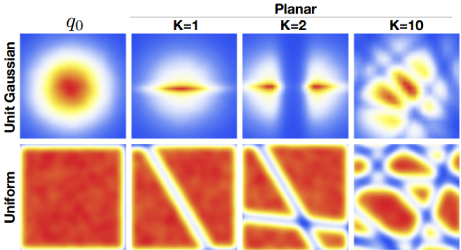
\includegraphics[scale=0.4]{pics/normflows.png} \\
\vspace{5mm}
(from \cite{Rezende2015})
\end{frame} 
\subsection{IWAE}
\begin{frame}
\thetitle{Importance Weighted Autoencoder (IWAE)~\citep{Burda2015}}
\begin{itemize}
    \item Flows are a way of tightening the ELBO by making the variational family more flexible. 
    \item Not the only way: can obtain a tighter lower bound on $\log p(x \param \theta)$ by using multiple importance samples.
\end{itemize}

    \air
    \air

    Consider:
    \begin{align*}
        I_K = \frac{1}{K} \sum_{k=1}^K \frac{p(x, z^{(k)} \param \theta)}{q(z^{(k)} \given x \param \lambda)},
    \end{align*}
    where each $z^{(k)} \sim q(z \given x \param \lambda)$.
    
    \air
    \air
    Note that $I_K$ is an unbiased estimator of $p(x \param \theta)$:
    \begin{align*}
        \E_{q(z^{(1:K)} \given x \param \lambda)} \left[I_K \right] = p(x \param \theta).
    \end{align*}

\air
% 
\end{frame}


\begin{frame}
\thetitle{Importance Weighted Autoencoder (IWAE)~\citep{Burda2015}}
    \textit{Any} unbiased estimator of $p(x \param \theta)$ can be used to obtain a lower bound, using Jensen's inequality:
    \begin{align*}
        p(x \param \theta) &= \E_{q(z^{(1:K)} \given x \param \lambda)} \left[ I_K \right] \\
        \implies \log p(x \param \theta) &\geq \E_{q(z^{(1:K)} \given x \param \lambda)} \left[ \log I_K \right] \\
        &= \E_{q(z^{(1:K)} \given x \param \lambda)} \left[ \log \frac{1}{K} \sum_{k=1}^K \frac{p(x, z^{(k)} \param \theta)}{q(z^{(k)} \given x \param \lambda)} \right]
    \end{align*}

However, can also show~\citep{Burda2015}:
\begin{itemize}
    \item $\log p(x \param \theta) \geq \E \left[ \log I_K \right] \geq \E \left[ \log I_{K-1} \right]$
    \item $\lim_{K \rightarrow \infty} \E \left[ \log I_K \right] = \log p(x \param \theta)$ under mild conditions
\end{itemize}
\end{frame}

\begin{frame}
\thetitle{Importance Weighted Autoencoder (IWAE)~\citep{Burda2015}}
\[ \E_{q(z^{(1:K)} \given x \param \lambda)} \left[ \log \frac{1}{K} \sum_{k=1}^K \frac{p(x, z^{(k)} \param \theta)}{q(z^{(k)} \given x \param \lambda)} \right] 
\]
    \begin{itemize}
      \item Note that with $K=1$, we recover the ELBO.
      \item Can interpret $\frac{p(x, z^{(k)} \param \theta)}{q(z^{(k)} \given x \param \lambda)}$ as importance weights.
        \item If $q(z \given x \param \lambda)$ is reparameterizable, we can use the reparameterization trick to optimize $\E \left[ \log I_K \right]$ directly.
        \item Otherwise, need score function gradient estimators \citep{Mnih2016}.
    \end{itemize}
\end{frame}


